El día de hoy se realizó el desarrollo teórico del problema de los tres péndulos físicos acoplados por resortes, donde el sistema es el siguiente:

\begin{figure}[htbp!]
  \centering
  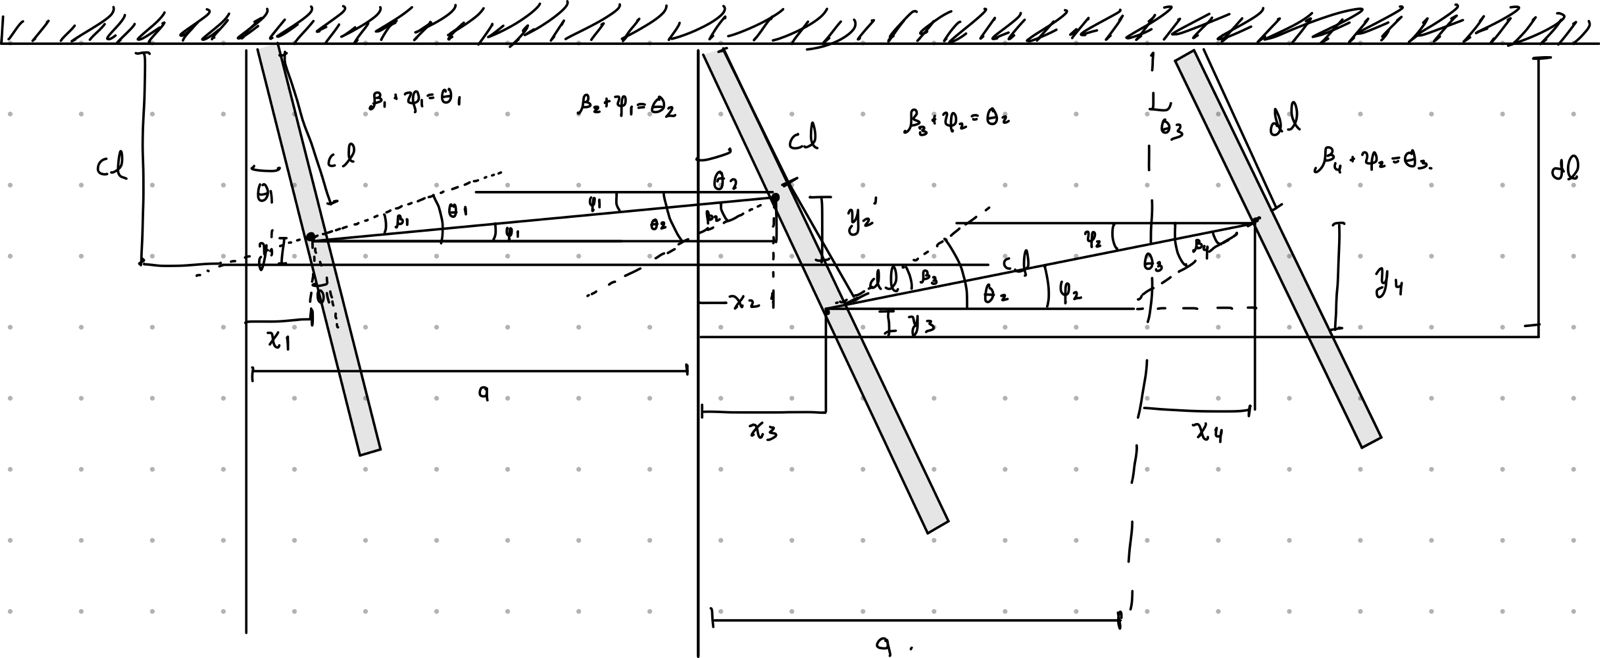
\includegraphics[width=0.8\linewidth]{Figures/IM1.jpeg}
  \caption{Sistema de tres péndulos físicos acoplados por resortes.}
  \label{fig:sistema_pendulos}
\end{figure}

Donde el resultado de la sumatoria de torques para cada péndulo genera el siguiente sistema de ecuaciones:

\begin{equation}
  \begin{aligned}
    \ddot{\theta}_1 =\; & \theta_1 \left( \frac{(cl)^2 - x_{cm1} m_1 g}{I_1} \right) + \theta_2 \left( -\frac{k_1 (cl)^2}{I_1} \right) \\
    \ddot{\theta}_2 =\; & \theta_1 \left( \frac{k_1 (cl)^2}{I_2} \right) + \theta_2 \left( -\frac{k_1 (cl)^2}{I_2} + \frac{k_2 (dl)^2}{I_2} + \frac{x_{cm2} m_2 g}{I_2} \right) + \theta_3 \left( \frac{k_2 (dl)^2}{I_2} \right) \\
    \ddot{\theta}_3 =\; & \theta_2 \left( \frac{k_2 (dl)^2}{I_3} \right) + \theta_3 \left( -\frac{k_2 (dl)^2}{I_3} - \frac{x_{cm3} m_3 g}{I_3} \right)
  \end{aligned}
\end{equation}

\vspace{ 0.5cm }


Adicionalmente, se hizo el planteamiento de cómo sería el montaje experimental. La idea es que se cumplan las siguientes condiciones:

\begin{itemize}
  \item Usar barras masivas, de modo que, en comparación con constantes elásticas bajas de los resortes, se obtengan series de tiempo extensas. Esto es importante, ya que en el caso real se tiene rozamiento con el aire y en las zonas de contacto (rodamientos).
  
  \item Utilizar resortes que se asemejen lo más posible al muelle ideal, es decir, completamente rectos entre los puntos de contacto. Esto se logra con constantes elásticas muy pequeñas. Además, es necesario que el resorte pueda comprimirse y expandirse ante fuerzas tanto compresivas como extensivas.
  
  \item Obtener barras "ideales", donde los puntos de contacto estén centrados y equidistantes en las tres barras.
\end{itemize}

La forma de lograr esto sería buscando barras muy masivas, hechas de un material de alta densidad, como algún metal, descartando en primera aproximación al aluminio por su baja densidad. Se planea que para la toma de datos se utilizarán sensores rotacionales angulares CASSY. Se acoplarán tres en serie, cada uno con una barra, ya que cada sensor está montado en un rodamiento que permite mayor libertad de movimiento y cuenta con un soporte del cual se pueden colgar los objetos que rotan.

\begin{figure}[htbp!]
  \centering
  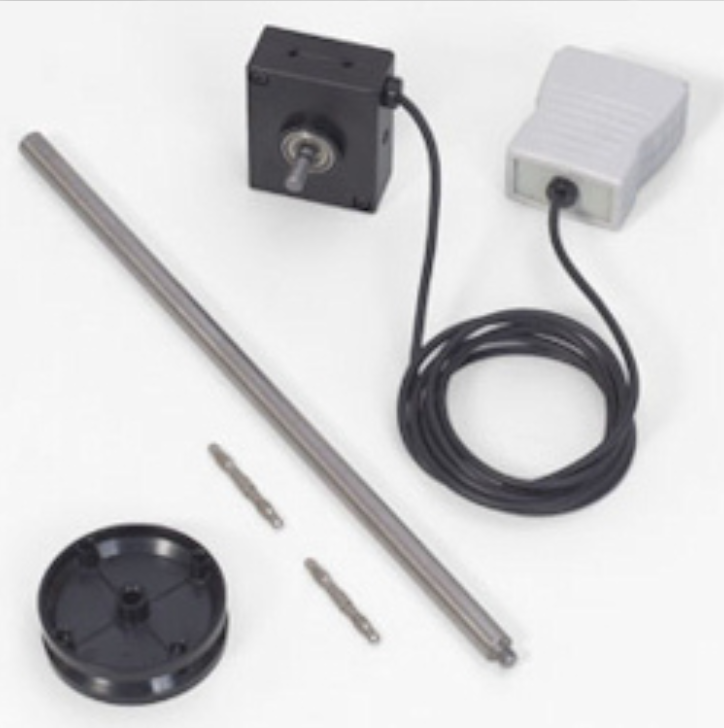
\includegraphics[width=0.8\linewidth]{Figures/IM2.png}
  \caption{Sensor CASSY de movimiento angular.}
  \label{fig:sistema_pendulos}
\end{figure}

